%%%%%%%%%%%%%%%%%%%%%%%%%%%%%%%%%%%%%%%%
% Uppsala University Assignment Title Page 
% LaTeX Template
% Version 1.0 (27/12/12)
%
% This template has been downloaded from:
% http://www.LaTeXTemplates.com
%
% Original author:
% WikiBooks (http://en.wikibooks.org/wiki/LaTeX/Title_Creation)
% Modified by Elsa Slattegard to fit Uppsala university
% License:
% CC BY-NC-SA 3.0 (http://creativecommons.org/licenses/by-nc-sa/3.0/)

%\title{Title page with logo}
%----------------------------------------------------------------------------------------
%	PACKAGES AND OTHER DOCUMENT CONFIGURATIONS
%----------------------------------------------------------------------------------------

\documentclass[12pt]{article}
\usepackage{longtable}
\usepackage[english]{babel}
\usepackage[utf8x]{inputenc}
\usepackage{amsmath}
\usepackage{amssymb}
\usepackage{url}
\usepackage{graphicx}
\usepackage{float}
\usepackage{multirow} % needed for tables
\usepackage{listings} % needed for code inclusion
\setlength {\marginparwidth}{2cm}
\usepackage[colorinlistoftodos]{todonotes}
\usepackage{xcolor}
\usepackage{caption}
\usepackage{subcaption}
\usepackage{algorithm}
\usepackage{algpseudocode}
\usepackage{float}

 % this chunk defines the colors for code inclusion
\lstset{
    language=C,
    basicstyle=\ttfamily\small,
    keywordstyle=\color{blue},
    stringstyle=\color{red},
    commentstyle=\color{purple},
    numbers=left,
    numberstyle=\tiny\color{gray},
    stepnumber=1,
    breaklines=true,
    frame=single,
    tabsize=4
}


\begin{document}

\begin{titlepage}

\newcommand{\HRule}{\rule{\linewidth}{0.5mm}} % Defines a new command for the horizontal lines, change thickness here

\center % Center everything on the page
 
%----------------------------------------------------------------------------------------
%	HEADING SECTIONS
%----------------------------------------------------------------------------------------

\textsc{\LARGE Uppsala University}\\[1.5cm] % Name of your university/college

\includegraphics[scale=.1]{Uppsala_University_seal_svg.png}\\[1cm] % Include a department/university logo - this will require the graphicx package
\textsc{\Large Accelerator-Based Programming}\\[0.5cm] % Major heading such as course name
\textsc{\large 1TD054}\\[0.5cm] % Minor heading such as course title

%----------------------------------------------------------------------------------------
%	TITLE SECTION
%----------------------------------------------------------------------------------------

\HRule \\[0.4cm]
{ \huge \bfseries Flash Attention Forward Pass}\\[0.4cm] % Title of your document
\HRule \\[1.5cm]
 
%----------------------------------------------------------------------------------------
%	AUTHOR SECTION
%----------------------------------------------------------------------------------------

\begin{minipage}{0.4\textwidth}
\begin{flushleft} \large
\emph{Authors:}\\
Anton \textsc{von Nandelstadh}\\% Your name
\end{flushleft}

\end{minipage}\\[2cm]

% If you don't want a supervisor, uncomment the two lines below and remove the section above
%\Large \emph{Author:}\\
%John \textsc{Smith}\\[3cm] % Your name

%----------------------------------------------------------------------------------------
%	DATE SECTION
%----------------------------------------------------------------------------------------

{\large Targeted grade: 5}\\[1cm]

{\large \today}\\[2cm] % Date, change the \today to a set date if you want to be precise

\vfill % Fill the rest of the page with whitespace

\end{titlepage}

\section{Background}
Multi-head attention is one of the core algorithms in the transformer model used in most modern large language models. Attention computes $O =$ softmax$(QK^T / \sqrt{d}) V$, where $Q, K$ and $V$ are $N \times d$ matrices ($N$ is the sequence length, $d$ the head dimension). The standard implementation writes the $N \times N$ score matrix $S = QK^T$ to global memory, applies a row-wise softmax and multiplies by $V$. This needs $O(N^2)$ extra memory, and the work is dominated by moving $S$ in and out of global memory. FlashAttention (FA)~\cite{dao2022flashattention} processes $Q, K$ and $V$ in tiles held in shared memory and uses an online softmax. These are dense matrices, produced by multiplying the input sequence with learned dense matrix weights. For each query row it keeps a running maximum and a running sum, and rescales the partial output whenever a new $K/V$ tile changes the maximum. $S$ is never written to global memory, so the memory footprint stays $O(Nd)$. FlashAttention2~\cite{dao2024flashattention2} improved upon this, by changing the loop order, freeing up some shared memory and thus allowing for higher arithmetic intensity.



\section{Method}


The forward pass implemented in \texttt{flash\_attention.cu} is given in Algorithm~\ref{alg:fa}. It follows the notation of Algorithm~1 of~\cite{dao2022flashattention}, but with the loop order of FlashAttention2~\cite{dao2024flashattention2}: each thread block owns one $Q_i$ and loops over all $K_j, V_j$, so $m_i$, $\ell_i$ and $O_i$ never leave the chip and the normalisation by $\ell_i$ is applied once at the end. Both matrix products run on tensor cores with FP16 inputs and FP32 accumulation. $B_r$ and $B_c$ are chosen to maximise the resident warps per SM within the shared memory, and the zero-padded tail of the last $K_j$ is masked to $-\infty$ in $S_{ij}$.

\begin{algorithm}[H]
\caption{FlashAttention forward pass (FA2 loop order)}
\label{alg:fa}
\begin{algorithmic}[1]
\Require Matrices $Q, K, V \in \mathbb{R}^{N \times d}$ in HBM, on-chip SRAM of size $M$, $\tau = 1/\sqrt{d}$.
\State Set block sizes $B_r, B_c$ for maximum occupancy within $M$.
\State Divide $Q$ into $T_r = \lceil N/B_r \rceil$ blocks $Q_1, \dots, Q_{T_r}$ of size $B_r \times d$ each, and divide $K, V$ into $T_c = \lceil N/B_c \rceil$ blocks $K_1, \dots, K_{T_c}$ and $V_1, \dots, V_{T_c}$ of size $B_c \times d$ each.
\State Divide $O$ into $T_r$ blocks $O_1, \dots, O_{T_r}$ of size $B_r \times d$ each.
\For{$1 \le i \le T_r$ \textbf{in parallel}}
    \State Load $Q_i$ from HBM to on-chip SRAM.
    \State On chip, initialize $O_i = (0)_{B_r \times d}$, $\ell_i = (0)_{B_r}$, $m_i = (-\infty)_{B_r}$.
    \For{$1 \le j \le T_c$}
        \State Load $K_j, V_j$ from HBM to on-chip SRAM.
        \State On chip, compute $S_{ij} = \tau Q_i K_j^T$, $m_i^{\text{new}} = \max(m_i, \operatorname{rowmax}(S_{ij}))$.
        \State On chip, compute $\tilde{P}_{ij} = \exp(S_{ij} - m_i^{\text{new}})$, $\ell_i \gets e^{m_i - m_i^{\text{new}}} \ell_i + \operatorname{rowsum}(\tilde{P}_{ij})$.
        \State On chip, compute $O_i \gets \operatorname{diag}(e^{m_i - m_i^{\text{new}}}) O_i + \tilde{P}_{ij} V_j$, $m_i \gets m_i^{\text{new}}$.
    \EndFor
    \State On chip, compute $O_i \gets \operatorname{diag}(\ell_i)^{-1} O_i$.
    \State Write $O_i$ to HBM.
\EndFor
\State \Return $O$.
\end{algorithmic}
\end{algorithm}

The scaffolding for the CUDA kernel is based on the flash-attention-minimal implementation of FA1~\cite{kim2024flashattentionminimal}, but the kernel itself is completely different. We highlight some key features of the code here. Below, we see how the $K_j$ and $V_j$ tiles are loaded into SRAM at each of the $T_c$ iterations of the inner for loop.


\begin{lstlisting}[language=C, caption={Loading $K_j$ and $V_j$ into shared memory.}]
for (int e = tx; e < KV_tile_size; e += blockDim.x){
	int KV_row = j*bc + e/d;
	bool in_bounds = KV_row < N;
	K_j[e] = __float2half(in_bounds ? K[matrix_offset + (KV_tile_size*j) + e]: 0.0f);
	V_j[e] = __float2half(in_bounds ? V[matrix_offset + (KV_tile_size*j) + e]: 0.0f);
}
__syncthreads();

int KV_valid = min(bc, N - j*bc);
\end{lstlisting}

Perhaps the main computation is that of $S_{ij}$. In order to speed up this computation, we use wmma to move it onto the tensor cores, which are optimised for matrix multiplication. This is seen below. The computation of $O_i$ is very similar and hence omitted.

\begin{lstlisting}[language=C, caption={Compute this warp's rows of $S_{ij} = Q_i*K_j^T$ on tensor cores
}]
for (int n = 0; n < bc; n += WN){
	wmma::fragment<wmma::accumulator, WM, WN, WK, float> acc;
	wmma::fill_fragment(acc, 0.0f);
	for (int k = 0; k < d; k += WK){
		wmma::fragment<wmma::matrix_a, WM, WN, WK, __half, wmma::col_major> Q_frag;
		wmma::fragment<wmma::matrix_b, WM, WN, WK, __half, wmma::col_major> K_frag;
		wmma::load_matrix_sync(Q_frag, &Q_i[k*br + r0], br);
		wmma::load_matrix_sync(K_frag, &K_j[n*d + k], d);
		wmma::mma_sync(acc, Q_frag, K_frag, acc);
	}
	wmma::store_matrix_sync(&S_ij[n*br + r0], acc, br, wmma::mem_col_major);
}
__syncwarp();

\end{lstlisting}

One of the key ideas of the original flash attention algorithms is to keep track of $\ell$ and $m$ in order so that we can parallelise the softmax. The computation of $P_{ij}$ using these principles is shown below.

\begin{lstlisting}[language=C, caption={Compute P (as half for the next MMA) and update the running sum
}]
float row_sum = 0.0f;
for (int y = y0; y < y1; y++){
	float p = __expf(S_ij[(y*br) + row] - row_max_new);
	P_ij[(y*br) + row] = __float2half(p);
	row_sum += p;
}
row_sum += __shfl_xor_sync(FULL_MASK, row_sum, 16);
float alpha = __expf(row_max - row_max_new); // Rescales everything accumulated so far
row_l = alpha*row_l + row_sum;
row_max = row_max_new;
\end{lstlisting}


In order to maximise occupancy, which we find to be our main bottleneck, we search the grid $(B_r, B_c)$ with values in $\{64, 128\} \times \{16, 32, 48, 64\}$ for the pair that maximises occupancy. We compute the shared bytes per block and then we query \texttt{cudaOccupancyMaxActiveBlocksPerMultiprocessor} and compare different values in the grid.

We have tried to improve access patterns as much as possible. Optimisations here include coalesced $Q$ and $K/V$ loading, and $O$ storage. This means that each warp instruction moves $128$ contiguous bytes and does not waste bandwidth. We also changed the order of dimensions to grid\_dim$(tr, nh, B)$, so that the $Q$ tiles are in the fastest-varying index x. Moreover, $S_{ij}$, $P_{ij}$ and $O_i$ are all stored in a column-major layout, due to how they are used in the kernel.

\section{Results}
Fig. \ref{Time} shows us how the time per forward pass grows quadratically with sequence length for the unfused and CPU kernels. However, we also see that the Flash Attention kernel with only one head grows linearly. This is because the GPU has not been saturated yet, but when the GPU is full as in the multi-head case, the growth becomes quadratic. Hence we see that the FA kernel is faster for all but the smallest batches. There is a kink in the unfused GPU kernel for single head runs when $S$ outgrows the L2 cache.

\begin{center}
\begin{minipage}{\textwidth}
\centering
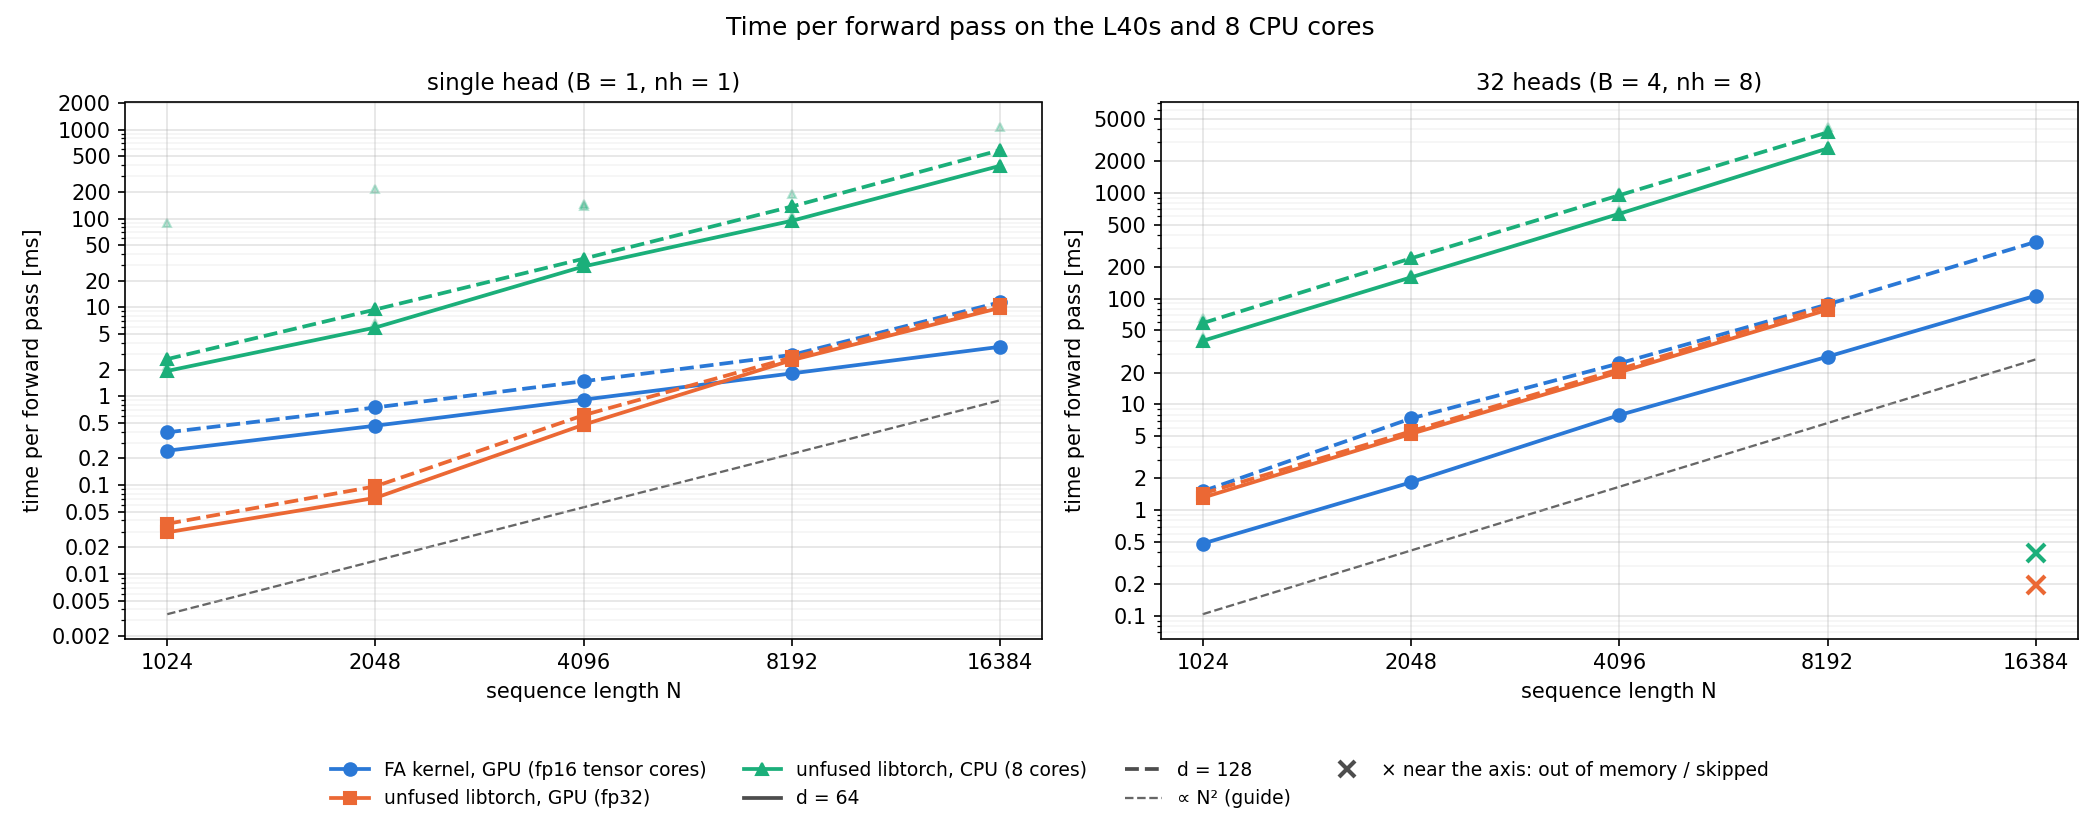
\includegraphics[width=\textwidth,height=0.8\textheight,keepaspectratio]{../figures/time.png}
\captionof{figure}{Time per forward pass versus the sequence length $N$ for a single head (left) and 32 heads (right), with $d = 64$ (solid) and $d = 128$ (dashed), for the FA kernel and unfused libtorch on the L40s and on 8 CPU cores.}
\label{Time}
\end{minipage}
\end{center}

In Fig. \ref{GFlops} we see the computational throughput for the different kernels. We find that the throughput of the FA kernel is roughly 50\% faster than the unfused kernel, when comparing optimal values of $d$. Both GPU kernels outperform the CPU kernel by several orders of magnitude. Nevertheless, even the FA kernel is very far from achieving optimal FLOPs. 

\begin{center}
\begin{minipage}{\textwidth}
\centering
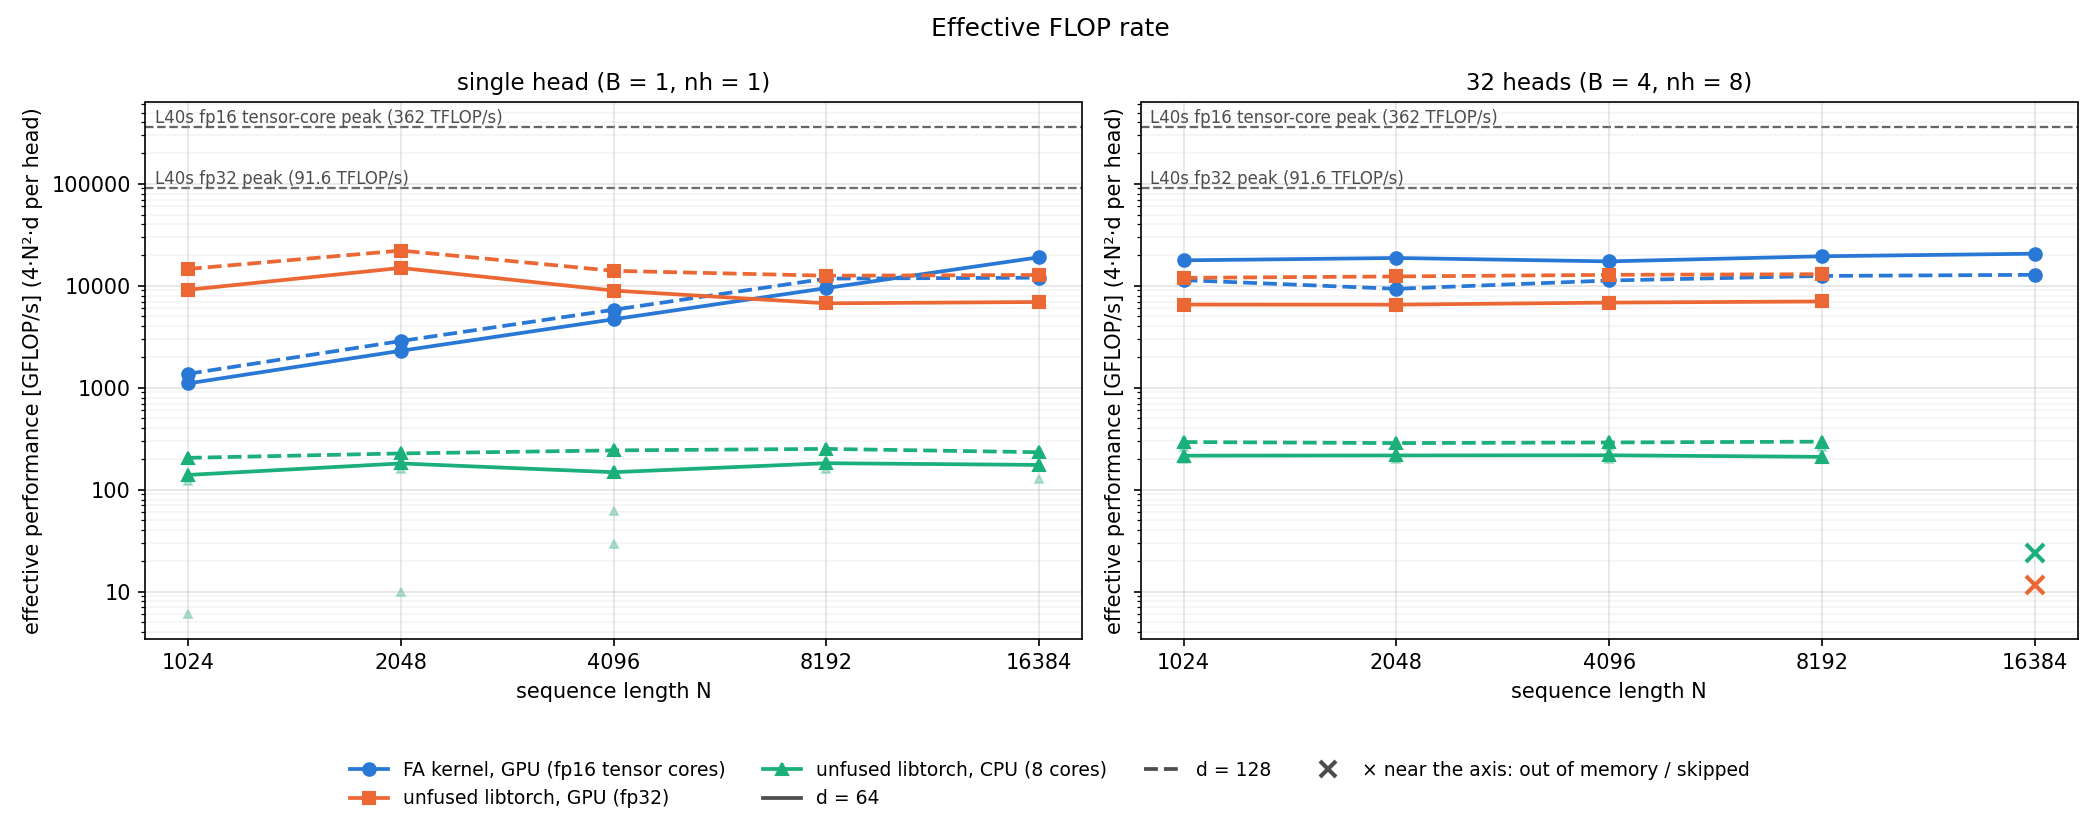
\includegraphics[width=\textwidth,height=0.8\textheight,keepaspectratio]{../figures/gflops.png}
\captionof{figure}{Effective floating point throughput ($4N^2d$ flops per head) versus $N$ for every implementation and head dimension, with the L40s fp32 and fp16 tensor-core peaks (dashed).}
\label{GFlops}
\end{minipage}
\end{center}

Fig. \ref{Speedup} shows the speedup of the FA kernel over the other kernels. It tells a similar story of the FA kernel outperforming for large batches. However, comparing $d=128$ embeddings, the fused and unfused kernels perform about the same, but this is because the FA kernel performs better at $d=64$.

\begin{center}
\begin{minipage}{\textwidth}
\centering
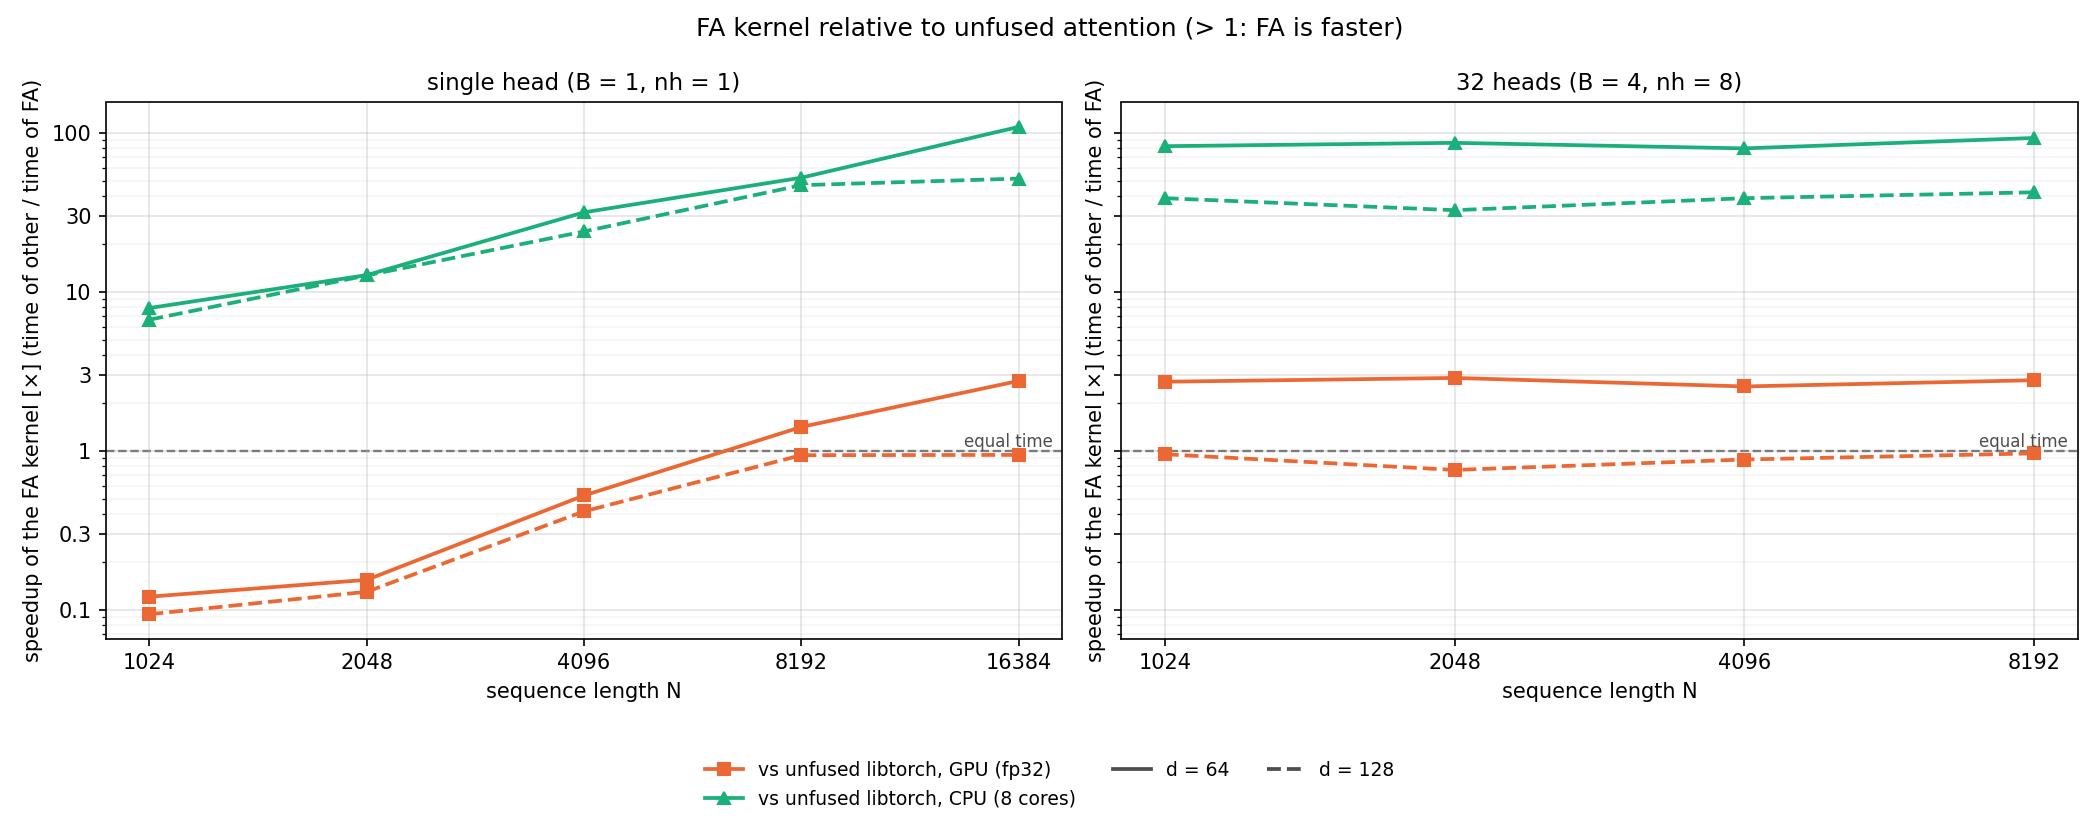
\includegraphics[width=\textwidth,height=0.8\textheight,keepaspectratio]{../figures/speedup.png}
\captionof{figure}{Speedup of the FA kernel over unfused libtorch on the GPU and on the CPU versus $N$; values above 1 mean the FA kernel is faster.}
\label{Speedup}
\end{minipage}
\end{center}

In Fig. \ref{Memory} we see a significant difference between the fused and unfused kernels. The fused kernel's memory usage grows linearly, while the others' grow quadratically. This is because the FA algorithm only stores tiles $S_{ij}$ in memory, and never the whole score matrix. Because of this the unfused kernels fail to complete for the largest batches.

\begin{center}
\begin{minipage}{\textwidth}
\centering
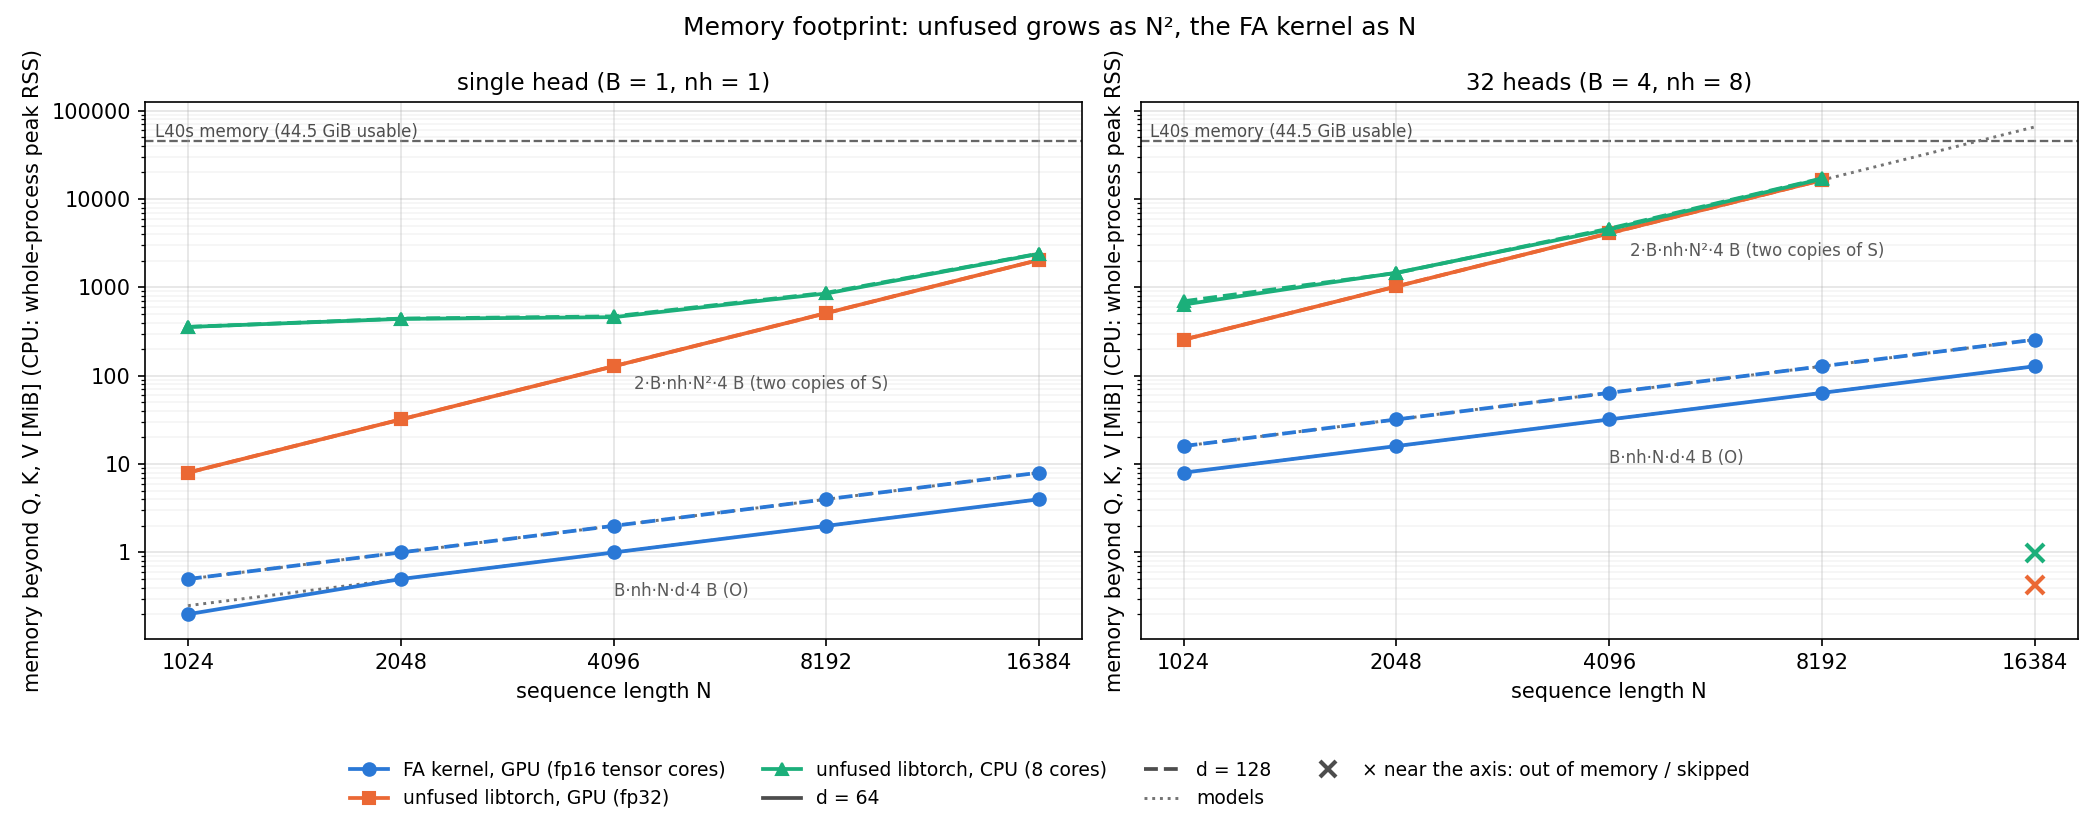
\includegraphics[width=\textwidth,height=0.8\textheight,keepaspectratio]{../figures/memory.png}
\captionof{figure}{Memory allocated beyond $Q$, $K$ and $V$ versus $N$ (CPU: whole-process peak RSS), with the models $2Bn_hN^2\cdot4$\,B for unfused and $Bn_hNd\cdot4$\,B for the FA kernel (dotted) and the usable L40s memory (dashed).}
\label{Memory}
\end{minipage}
\end{center}

Fig. \ref{Traffic} shows the DRAM traffic per forward pass, taken from Nsight Compute. DRAM traffic for the unfused kernel grows quadratically, while for the fused kernel it grows linearly. This is because the unfused kernel reads $S$ at every pass, whereas the fused kernel reads the matrices only once into SRAM.

\begin{center}
\begin{minipage}{\textwidth}
\centering
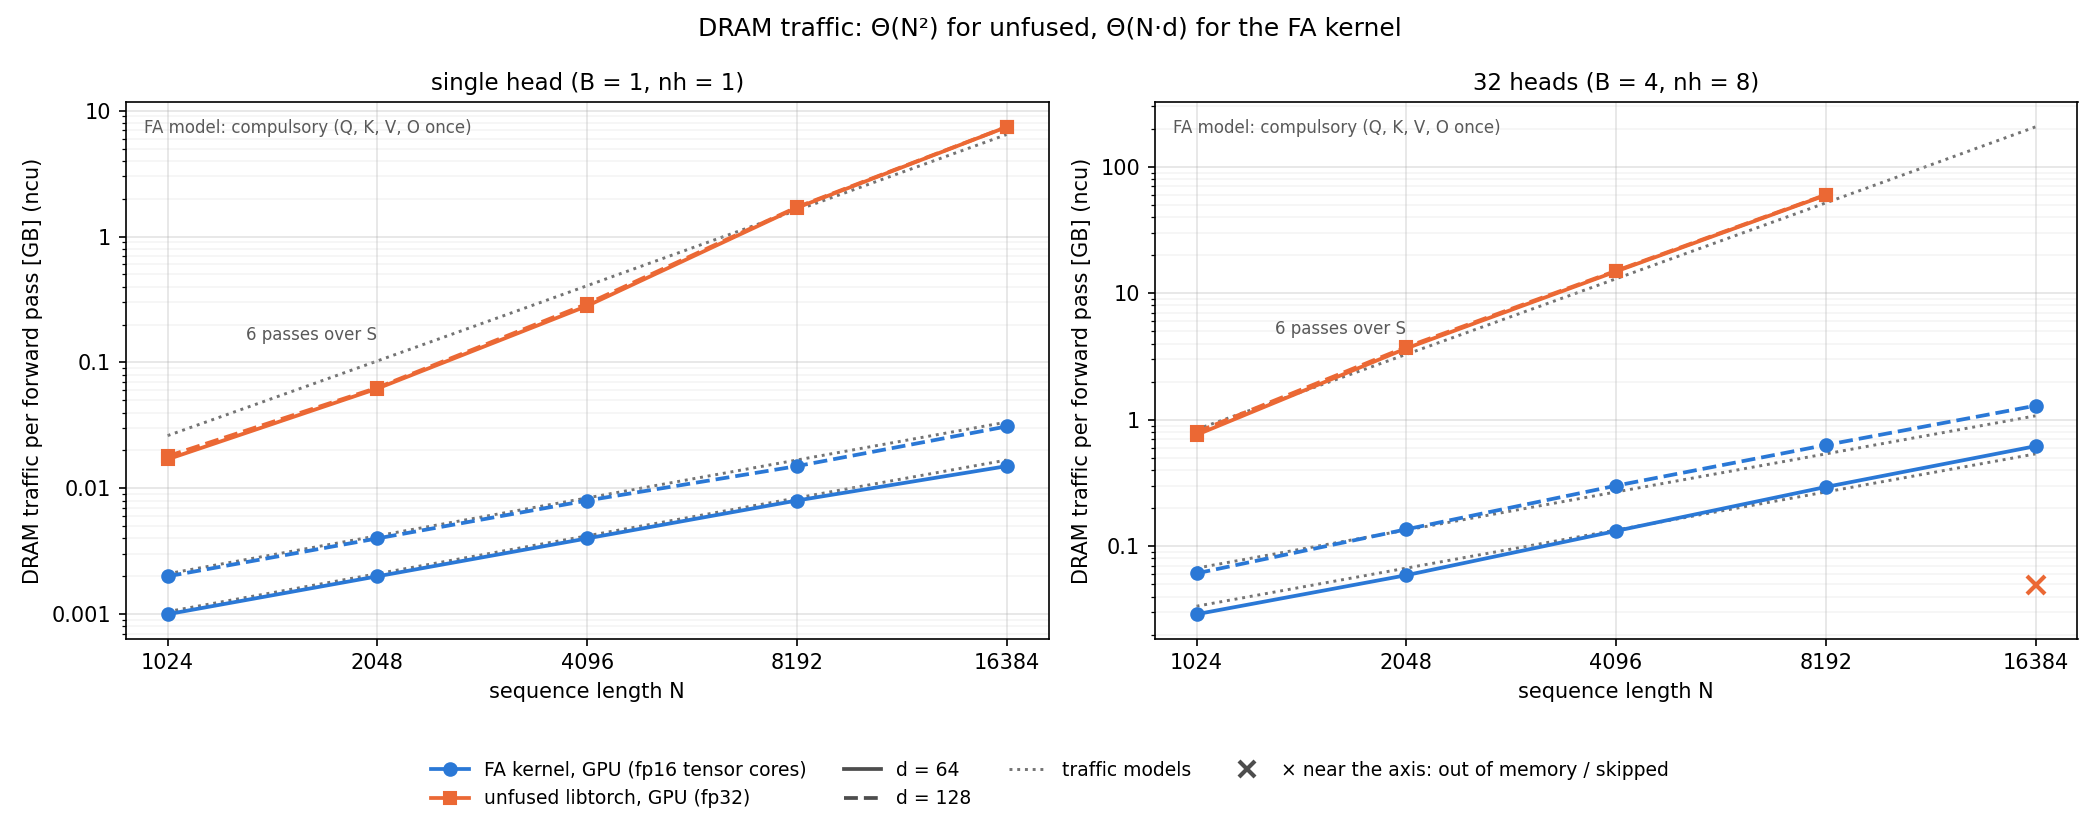
\includegraphics[width=\textwidth,height=0.8\textheight,keepaspectratio]{../figures/dram_traffic.png}
\captionof{figure}{DRAM traffic per forward pass measured with Nsight Compute versus $N$, with the traffic models (dotted).}
\label{Traffic}
\end{minipage}
\end{center}

Fig. \ref{Bandwidth} shows the amount of DRAM bandwidth used for the different GPU kernels. We see that the unfused kernel is clearly bandwidth bound, whereas this ceases to be the case for the fused kernel.

\begin{center}
\begin{minipage}{\textwidth}
\centering
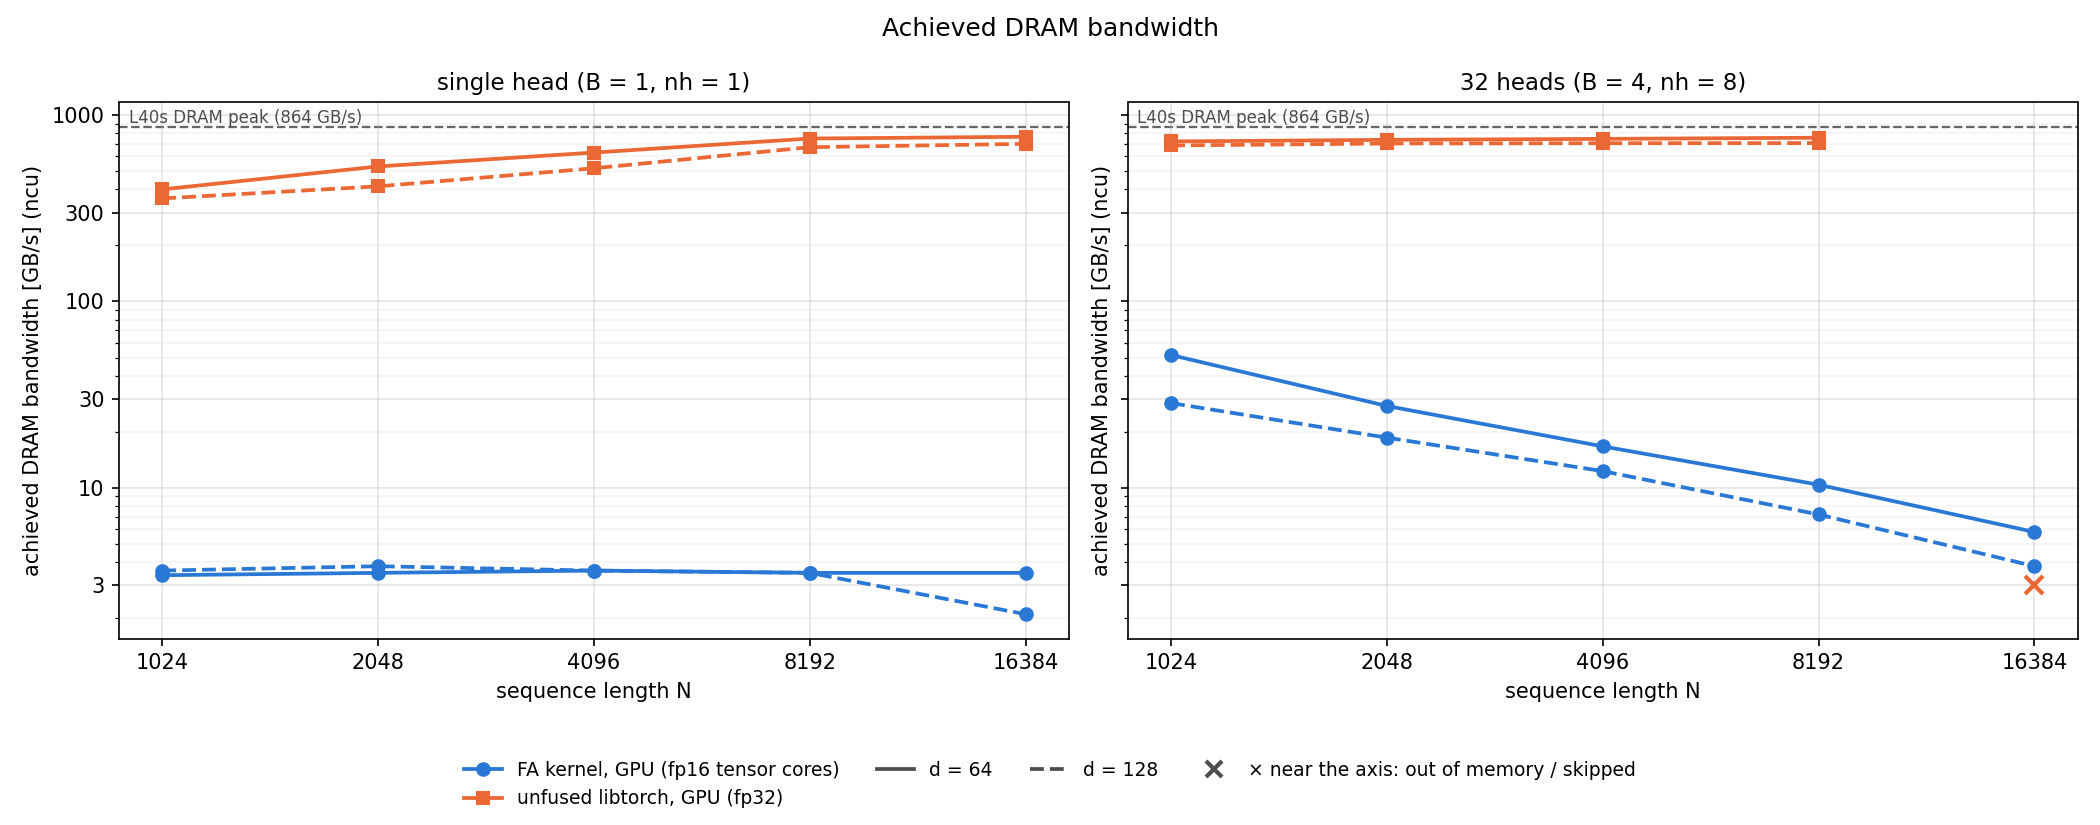
\includegraphics[width=\textwidth,height=0.8\textheight,keepaspectratio]{../figures/bandwidth.png}
\captionof{figure}{Achieved DRAM bandwidth versus $N$ for the GPU implementations, with the L40s DRAM peak of 864\,GB/s (dashed).}
\label{Bandwidth}
\end{minipage}
\end{center}

Fig. \ref{Roofline} is a roofline model, with the unfused kernel in orange, and the fused kernel in blue. It neatly illustrates how the unfused kernel is memory-bound, while the fused kernel is not.

\begin{center}
\begin{minipage}{\textwidth}
\centering
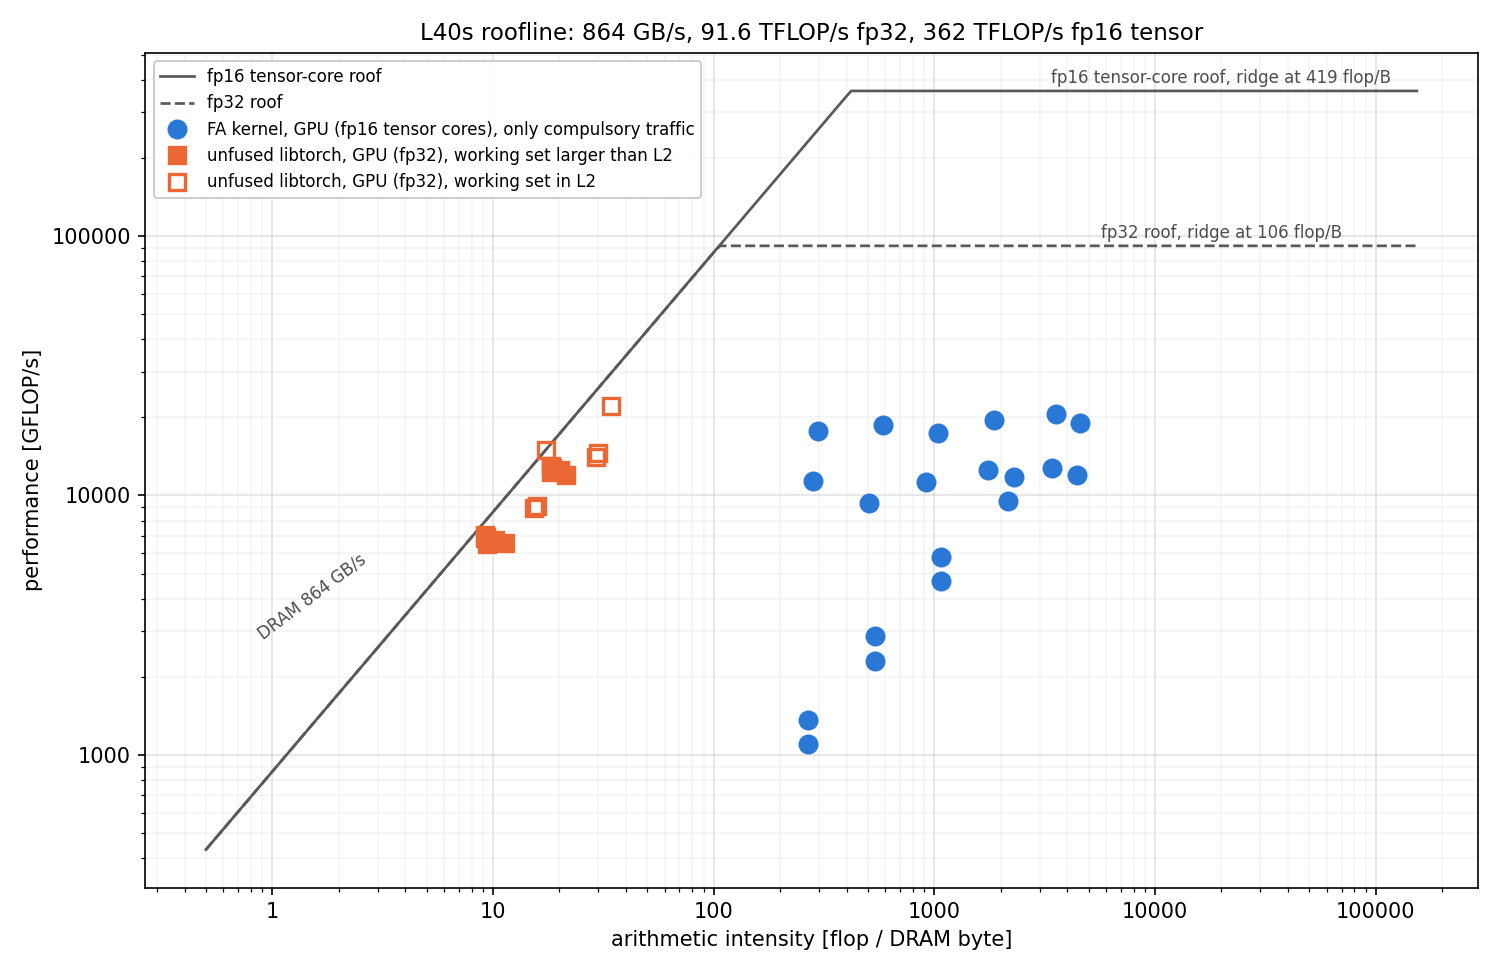
\includegraphics[width=\textwidth,height=0.8\textheight,keepaspectratio]{../figures/roofline.png}
\captionof{figure}{Roofline model of the L40s with the fp32 and fp16 tensor-core ceilings and every GPU measurement; hollow markers are runs whose working set fits in L2, which inflates their arithmetic intensity.}
\label{Roofline}
\end{minipage}
\end{center}

\section{Discussion}
The results above clearly motivate the need for a fused attention kernel. The CPU kernel is incredibly slow compared with even the unfused GPU kernel, as the 8 threads we ran it on cannot match the 18176 cores of the L40 GPU. Nevertheless, the roofline model and bandwidth analysis show that the unfused GPU kernel completely saturates DRAM bandwidth. Hence the fused kernel from the FlashAttention algorithm outperforms the unfused kernel by not constantly loading $S$ into HBM, but rather by working on tiles $S_{ij}$ kept in SRAM. This removes the bandwidth bound, but creates a new bound, which is the size of SRAM. Because only a few blocks saturate SRAM, we cannot use the full FLOP capacity per SM, and hence stay quite far from the theoretical tensor core FLOPs. One way to improve on this is to follow FA2, which keeps e.g. $O_i$ in registers instead of in SRAM. However, we did not implement this as it increases code complexity quite significantly.

Because our new performance bound is SRAM size, the tile sizes we use matter. This is likely why $d=128$ performs worse than $d=64$, since $d=128$ constrains the size of the tiles more. The way we choose tile sizes i.e. $B_r$ and $B_c$ in the algorithm, is by dynamically checking what saturates SRAM. Hence we cannot be sure that the tiles are completely optimal, but we do know that they are optimal within the grid searched.

For access patterns, we implemented multiple optimisations described above. However, this does not seem to be the bottleneck in our case, but rather occupancy as described above is. We get $8$ warps per SM for $d=64$ and $4$ warps per SM for $d=128$, out of a possible $48$.

A Flash Attention implementation on a framework such as Kokkos would inherently suffer from the higher level of abstraction required by such a framework. The way we would map this to Kokkos is by using a league of teams for a grid of blocks, teams for blocks and level-0 team scratch for shared memory. However, there are significant limitations. Access to tensor cores or syncing warps on a low level, does not work well in Kokkos. It is additionally harder to query for specific hardware features, such as SM occupancy. 

\section{Conclusion}
We managed to get a significant performance improvement using our fused Flash Attention kernel, over the unfused kernel. Both massively outperform the CPU. We found that the bottleneck shifts from memory bandwidth to SRAM, as we fuse the kernel to minimise HBM access. Nevertheless, due to the brevity of this project, there were many optimisations which we did not have time to implement. The main one would be heavier usage of registers, which would decrease the pressure on SRAM. For newer generations of GPUs, there are also many other tricks you can use, detailed in FlashAttention-3~\cite{shah2024flashattention3} and FlashAttention-4~\cite{zadouri2026flashattention4}, designed for H100 and B200 respectively.

\section{AI Declaration}
Auxiliary code such as the testing harness, scripts, plots and tables were planned and generated with the help of Claude Code and Opus 5.5. The focus of human attention was on writing and understanding the core kernels and writing the report.

\bibliographystyle{unsrt}
\bibliography{references}

% generated by make_appendix.py -- do not edit by hand
\clearpage
\appendix
\section{Measurement tables}\label{app:tables}
\sloppy

This appendix lists every measurement behind the figures. Each configuration $(B, n_h, N, d)$ runs in its own process on random single-precision inputs. The attention is computed once as an untimed warm-up and once more to calibrate; then $n = \min(100, \max(1, \lfloor 1000\,\text{ms}/t_\text{cal} \rfloor))$ calls are timed together (for $n = 1$ the calibration call is the measurement), and $t$ is the average time of one call. GPU calls are timed with CUDA events and include the small kernels that allocate and initialise the output; CPU calls are timed with \texttt{std::chrono::steady\_clock}. GFLOP/s counts $4 B n_h N^2 d$ flops. Memory is the peak allocated by the libtorch caching allocator during one further call minus what was allocated before it ($Q$, $K$, $V$ and the cuBLAS workspace). DRAM traffic comes from a separate run in which Nsight Compute profiles only that one call: \texttt{dram\_\_bytes\_read.sum} plus \texttt{dram\_\_bytes\_write.sum} over all of its kernels, divided by their summed durations for the bandwidth. Occupancy is \texttt{sm\_\_warps\_active.avg.pct\_of\_peak\_sustained\_active}, weighted by kernel duration; it was only recorded for the final FA kernel. GPU runs used one NVIDIA L40s (48\,GB); CPU runs used 8 CPUs of a Pelle node (Slurm \texttt{-c 8}, 8 OpenMP threads, 32\,GB), and each CPU entry is the fastest of the available runs. Configurations whose unfused score matrices do not fit are marked out of memory or skipped.

\subsection{Correctness}

The FA kernel is compared with unfused libtorch attention on the GPU, using standard-normal random $Q$, $K$ and $V$, for a single head ($B = n_h = 1$) and a batch of heads ($B = 2$, $n_h = 4$), with $d \in \{32, 64, 128\}$ and $N \in \{1, 63, 64, 65, 1000, 4096\}$. Every candidate tile size is a multiple of 16, so $N = 1$ is smaller than any tile, and $N = 1$, 63, 65 and 1000 always leave the last $Q$ tile and the last $K/V$ tile partially filled. This exercises the zero padding and the masking of the padded scores. $N = 4096$ is a multiple of both candidate $B_r$, so every $Q$ tile is full. A configuration passes when \texttt{torch::allclose} holds with relative and absolute tolerance $5\cdot10^{-3}$, which allows for the fp16 inputs of the tensor-core products. Data from \texttt{results/test\_gpu\_7219777.log}.

\begingroup\footnotesize
\setlength{\tabcolsep}{2.5pt}
\renewcommand{\arraystretch}{1.2}
\begin{longtable}{rrrrrr}
\caption{Correctness of the FA kernel against unfused libtorch on the GPU.}\label{tab:test}\\
\hline
$B$ & $n_h$ & $N$ & $d$ & max $|O - O_\text{ref}|$ & result \\
\hline
\endfirsthead
\multicolumn{6}{l}{\emph{Table \thetable{} continued}}\\
\hline
$B$ & $n_h$ & $N$ & $d$ & max $|O - O_\text{ref}|$ & result \\
\hline
\endhead
\hline
\endfoot
1 & 1 & 1 & 32 & $3.99e-4$ & PASS \\
1 & 1 & 63 & 32 & $4.12e-4$ & PASS \\
1 & 1 & 64 & 32 & $4.13e-4$ & PASS \\
1 & 1 & 65 & 32 & $7.08e-4$ & PASS \\
1 & 1 & 1\,000 & 32 & $1.76e-4$ & PASS \\
1 & 1 & 4\,096 & 32 & $1.26e-4$ & PASS \\
1 & 1 & 1 & 64 & $8.39e-4$ & PASS \\
1 & 1 & 63 & 64 & $4.68e-4$ & PASS \\
1 & 1 & 64 & 64 & $4.02e-4$ & PASS \\
1 & 1 & 65 & 64 & $5.54e-4$ & PASS \\
1 & 1 & 1\,000 & 64 & $1.53e-4$ & PASS \\
1 & 1 & 4\,096 & 64 & $9.18e-5$ & PASS \\
1 & 1 & 1 & 128 & $9.69e-4$ & PASS \\
1 & 1 & 63 & 128 & $4.59e-4$ & PASS \\
1 & 1 & 64 & 128 & $7.17e-4$ & PASS \\
1 & 1 & 65 & 128 & $4.60e-4$ & PASS \\
1 & 1 & 1\,000 & 128 & $1.53e-4$ & PASS \\
1 & 1 & 4\,096 & 128 & $8.60e-5$ & PASS \\
2 & 4 & 1 & 32 & $9.13e-4$ & PASS \\
2 & 4 & 63 & 32 & $6.83e-4$ & PASS \\
2 & 4 & 64 & 32 & $6.33e-4$ & PASS \\
2 & 4 & 65 & 32 & $5.28e-4$ & PASS \\
2 & 4 & 1\,000 & 32 & $2.56e-4$ & PASS \\
2 & 4 & 4\,096 & 32 & $2.46e-4$ & PASS \\
2 & 4 & 1 & 64 & $9.56e-4$ & PASS \\
2 & 4 & 63 & 64 & $6.77e-4$ & PASS \\
2 & 4 & 64 & 64 & $6.54e-4$ & PASS \\
2 & 4 & 65 & 64 & $6.25e-4$ & PASS \\
2 & 4 & 1\,000 & 64 & $1.86e-4$ & PASS \\
2 & 4 & 4\,096 & 64 & $2.15e-4$ & PASS \\
2 & 4 & 1 & 128 & $8.85e-4$ & PASS \\
2 & 4 & 63 & 128 & $7.67e-4$ & PASS \\
2 & 4 & 64 & 128 & $8.02e-4$ & PASS \\
2 & 4 & 65 & 128 & $6.92e-4$ & PASS \\
2 & 4 & 1\,000 & 128 & $2.01e-4$ & PASS \\
2 & 4 & 4\,096 & 128 & $1.16e-4$ & PASS \\
\end{longtable}
\endgroup

\clearpage
\subsection{FA kernel, GPU (fp16 tensor cores)}

\begingroup\footnotesize
\setlength{\tabcolsep}{2.5pt}
\renewcommand{\arraystretch}{1.2}
\begin{longtable}{rrrrrrrrrr}
\caption{FA kernel, GPU (fp16 tensor cores), NVIDIA L40s. Mem.: memory beyond the inputs; DRAM and GB/s: traffic and achieved bandwidth from Nsight Compute; occ.: achieved occupancy.}\label{tab:fa}\\
\hline
$B\times n_h$ & $N$ & $d$ & $n$ & $t$ [ms] & GFLOP/s & mem. [MiB] & DRAM [GB] & GB/s & occ. [\%] \\
\hline
\endfirsthead
\multicolumn{10}{l}{\emph{Table \thetable{} continued}}\\
\hline
$B\times n_h$ & $N$ & $d$ & $n$ & $t$ [ms] & GFLOP/s & mem. [MiB] & DRAM [GB] & GB/s & occ. [\%] \\
\hline
\endhead
\hline
\endfoot
$1\times1$ & 1\,024 & 64 & 100 & 0.244 & 1\,101.0 & 0.2 & 0.001 & 3.4 & 16.7 \\
$1\times1$ & 2\,048 & 64 & 100 & 0.466 & 2\,302.2 & 0.5 & 0.002 & 3.5 & 16.7 \\
$1\times1$ & 4\,096 & 64 & 100 & 0.916 & 4\,688.4 & 1.0 & 0.004 & 3.6 & 16.7 \\
$1\times1$ & 8\,192 & 64 & 100 & 1.810 & 9\,492.1 & 2.0 & 0.008 & 3.5 & 16.7 \\
$1\times1$ & 16\,384 & 64 & 100 & 3.607 & 19\,053.4 & 4.0 & 0.015 & 3.5 & 16.7 \\
$1\times1$ & 1\,024 & 128 & 100 & 0.392 & 1\,368.6 & 0.5 & 0.002 & 3.6 & 8.3 \\
$1\times1$ & 2\,048 & 128 & 100 & 0.748 & 2\,869.6 & 1.0 & 0.004 & 3.8 & 8.3 \\
$1\times1$ & 4\,096 & 128 & 100 & 1.476 & 5\,818.0 & 2.0 & 0.008 & 3.6 & 8.3 \\
$1\times1$ & 8\,192 & 128 & 100 & 2.921 & 11\,761.1 & 4.0 & 0.015 & 3.5 & 8.3 \\
$1\times1$ & 16\,384 & 128 & 87 & 11.447 & 12\,006.8 & 8.0 & 0.031 & 2.1 & 8.3 \\
$4\times8$ & 1\,024 & 64 & 100 & 0.484 & 17\,757.8 & 8.0 & 0.029 & 51.6 & 16.7 \\
$4\times8$ & 2\,048 & 64 & 100 & 1.834 & 18\,733.5 & 16.0 & 0.059 & 27.5 & 16.7 \\
$4\times8$ & 4\,096 & 64 & 100 & 7.925 & 17\,343.0 & 32.0 & 0.132 & 16.7 & 16.7 \\
$4\times8$ & 8\,192 & 64 & 35 & 28.228 & 19\,475.3 & 64.0 & 0.294 & 10.4 & 16.7 \\
$4\times8$ & 16\,384 & 64 & 9 & 106.558 & 20\,636.9 & 128.0 & 0.618 & 5.8 & 16.7 \\
$4\times8$ & 1\,024 & 128 & 100 & 1.511 & 11\,368.5 & 16.0 & 0.061 & 28.5 & 8.3 \\
$4\times8$ & 2\,048 & 128 & 100 & 7.359 & 9\,338.1 & 32.0 & 0.136 & 18.6 & 8.3 \\
$4\times8$ & 4\,096 & 128 & 40 & 24.404 & 11\,263.7 & 64.0 & 0.301 & 12.3 & 8.3 \\
$4\times8$ & 8\,192 & 128 & 11 & 88.039 & 12\,489.0 & 128.0 & 0.631 & 7.2 & 8.3 \\
$4\times8$ & 16\,384 & 128 & 2 & 343.418 & 12\,806.7 & 256.0 & 1.291 & 3.8 & 8.3 \\
\end{longtable}
\endgroup

\clearpage
\subsection{Unfused libtorch, GPU (fp32)}

\begingroup\footnotesize
\setlength{\tabcolsep}{2.5pt}
\renewcommand{\arraystretch}{1.2}
\begin{longtable}{rrrrrrrrr}
\caption{Unfused libtorch, GPU (fp32), NVIDIA L40s. Mem.: memory beyond the inputs; DRAM and GB/s: traffic and achieved bandwidth from Nsight Compute.}\label{tab:unfused}\\
\hline
$B\times n_h$ & $N$ & $d$ & $n$ & $t$ [ms] & GFLOP/s & mem. [MiB] & DRAM [GB] & GB/s \\
\hline
\endfirsthead
\multicolumn{9}{l}{\emph{Table \thetable{} continued}}\\
\hline
$B\times n_h$ & $N$ & $d$ & $n$ & $t$ [ms] & GFLOP/s & mem. [MiB] & DRAM [GB] & GB/s \\
\hline
\endhead
\hline
\endfoot
$1\times1$ & 1\,024 & 64 & 100 & 0.029 & 9\,127.6 & 8.0 & 0.017 & 399.1 \\
$1\times1$ & 2\,048 & 64 & 100 & 0.072 & 14\,960.4 & 32.0 & 0.062 & 529.9 \\
$1\times1$ & 4\,096 & 64 & 100 & 0.479 & 8\,969.1 & 128.0 & 0.281 & 629.1 \\
$1\times1$ & 8\,192 & 64 & 100 & 2.554 & 6\,727.8 & 512.0 & 1.691 & 748.1 \\
$1\times1$ & 16\,384 & 64 & 100 & 9.912 & 6\,932.8 & 2\,048.0 & 7.411 & 764.6 \\
$1\times1$ & 1\,024 & 128 & 100 & 0.037 & 14\,616.3 & 8.0 & 0.018 & 357.0 \\
$1\times1$ & 2\,048 & 128 & 100 & 0.097 & 22\,152.2 & 32.0 & 0.063 & 414.4 \\
$1\times1$ & 4\,096 & 128 & 100 & 0.613 & 14\,011.4 & 128.0 & 0.292 & 518.1 \\
$1\times1$ & 8\,192 & 128 & 100 & 2.738 & 12\,550.7 & 512.0 & 1.711 & 672.1 \\
$1\times1$ & 16\,384 & 128 & 92 & 10.768 & 12\,763.1 & 2\,048.0 & 7.428 & 700.5 \\
$4\times8$ & 1\,024 & 64 & 100 & 1.313 & 6\,539.7 & 256.0 & 0.759 & 721.6 \\
$4\times8$ & 2\,048 & 64 & 100 & 5.263 & 6\,528.4 & 1\,024.0 & 3.666 & 736.2 \\
$4\times8$ & 4\,096 & 64 & 49 & 20.098 & 6\,838.4 & 4\,096.0 & 14.870 & 744.9 \\
$4\times8$ & 8\,192 & 64 & 12 & 78.363 & 7\,015.5 & 16\,384.0 & 59.622 & 755.6 \\
$4\times8$ & 16\,384 & 64 & \multicolumn{6}{l}{out of memory} \\
$4\times8$ & 1\,024 & 128 & 100 & 1.436 & 11\,963.4 & 256.0 & 0.798 & 686.4 \\
$4\times8$ & 2\,048 & 128 & 100 & 5.567 & 12\,343.5 & 1\,024.0 & 3.757 & 703.7 \\
$4\times8$ & 4\,096 & 128 & 46 & 21.476 & 12\,799.6 & 4\,096.0 & 15.041 & 705.9 \\
$4\times8$ & 8\,192 & 128 & 11 & 84.656 & 12\,988.0 & 16\,384.0 & 60.072 & 706.8 \\
$4\times8$ & 16\,384 & 128 & \multicolumn{6}{l}{out of memory} \\
\end{longtable}
\endgroup

\clearpage
\subsection{Unfused libtorch, CPU (8 cores)}

\begingroup\footnotesize
\setlength{\tabcolsep}{2.5pt}
\renewcommand{\arraystretch}{1.2}
\begin{longtable}{rrrrrrr}
\caption{Unfused libtorch, CPU (8 cores).}\label{tab:cpu}\\
\hline
$B\times n_h$ & $N$ & $d$ & $n$ & $t$ [ms] & GFLOP/s & peak RSS [MiB] \\
\hline
\endfirsthead
\multicolumn{7}{l}{\emph{Table \thetable{} continued}}\\
\hline
$B\times n_h$ & $N$ & $d$ & $n$ & $t$ [ms] & GFLOP/s & peak RSS [MiB] \\
\hline
\endhead
\hline
\endfoot
$1\times1$ & 1\,024 & 64 & 100 & 1.926 & 139.4 & 356.3 \\
$1\times1$ & 2\,048 & 64 & 100 & 5.938 & 180.8 & 440.0 \\
$1\times1$ & 4\,096 & 64 & 35 & 28.953 & 148.3 & 459.9 \\
$1\times1$ & 8\,192 & 64 & 10 & 94.503 & 181.8 & 853.1 \\
$1\times1$ & 16\,384 & 64 & 2 & 393.197 & 174.8 & 2\,400.6 \\
$1\times1$ & 1\,024 & 128 & 100 & 2.618 & 205.1 & 356.9 \\
$1\times1$ & 2\,048 & 128 & 16 & 9.478 & 226.6 & 443.2 \\
$1\times1$ & 4\,096 & 128 & 28 & 35.376 & 242.8 & 469.8 \\
$1\times1$ & 8\,192 & 128 & 7 & 136.832 & 251.1 & 869.5 \\
$1\times1$ & 16\,384 & 128 & 1 & 590.017 & 232.9 & 2\,414.4 \\
$4\times8$ & 1\,024 & 64 & 16 & 39.859 & 215.5 & 638.9 \\
$4\times8$ & 2\,048 & 64 & 6 & 158.643 & 216.6 & 1\,464.3 \\
$4\times8$ & 4\,096 & 64 & 1 & 632.492 & 217.3 & 4\,525.4 \\
$4\times8$ & 8\,192 & 64 & 1 & 2\,620.704 & 209.8 & 16\,922.9 \\
$4\times8$ & 16\,384 & 64 & \multicolumn{4}{l}{skipped (does not fit in the job's memory)} \\
$4\times8$ & 1\,024 & 128 & 15 & 58.621 & 293.1 & 696.3 \\
$4\times8$ & 2\,048 & 128 & 4 & 239.924 & 286.4 & 1\,453.2 \\
$4\times8$ & 4\,096 & 128 & 1 & 946.398 & 290.4 & 4\,630.0 \\
$4\times8$ & 8\,192 & 128 & 1 & 3\,718.832 & 295.7 & 17\,120.1 \\
$4\times8$ & 16\,384 & 128 & \multicolumn{4}{l}{skipped (does not fit in the job's memory)} \\
\end{longtable}
\endgroup

\end{document}

